% Copyright 2012 Alex Legler <alex@a3li.li>
% License: Creative Commons Attribution-ShareAlike 4.0 International (http://creativecommons.org/licenses/by-sa/4.0/)
\documentclass[svgnames]{beamer}

\usepackage[utf8]{inputenc}
\usepackage[default,scale=0.95]{opensans}
\usepackage[T1]{fontenc}
\usepackage{fancyvrb}
\usepackage{textcomp}
\renewcommand*\ttdefault{txtt}

\usepackage{tikz} 
\usetikzlibrary{arrows,decorations.pathmorphing,backgrounds,fit,positioning,shapes,chains}
\usepackage{pgfplots}

\definecolor{uniwueorange}{HTML}{F7800A}
\definecolor{uniwuegray}{HTML}{000000}
\definecolor{uniwuelightgray}{HTML}{D4D4D5}
\definecolor{uniwueblue}{HTML}{1F5394}

\usetheme[compress]{Gentoo}

\title{\textbf{Keeping Gentoo Secure}}
\subtitle{Open Source Security and how Gentoo does it}
\author{Alex Legler \texttt{<a3li@gentoo.org>}}
\institute{Gentoo Linux Security Team}
\date{Gentoo Miniconf Prague\\October 2012}
\logo{
\includegraphics[width=0.3\paperwidth]{img/bg.png}}

\newenvironment{changemargin}[2]{% 
  \begin{list}{}{% 
    \setlength{\topsep}{0pt}% 
    \setlength{\leftmargin}{#1}% 
    \setlength{\rightmargin}{#2}% 
    \setlength{\listparindent}{\parindent}% 
    \setlength{\itemindent}{\parindent}% 
    \setlength{\parsep}{\parskip}% 
  }% 
  \item[]}{\end{list}} 

\begin{document}
\setbeamercovered{dynamic}

\section{Introduction}
\subsection*{Introduction}

\begin{frame}
  \titlepage
\end{frame}

\begin{frame}
  \tableofcontents
\end{frame}

\begin{frame}
  \frametitle{Hi!}
  
  \begin{itemize}\addtolength{\itemsep}{1\baselineskip}
    \item \textbf{I'm Alex \textit{'a3li'} Legler}
    \item Living and studying in Würzburg, Germany
    \item Gentoo developer since 2009
    \begin{itemize}
      \item Involved in Ruby packaging, Security, Infra and PR
      \item Board member of the Gentoo e.V. association in Germany
      \item wiki.gentoo.org is mostly my fault
      \item Currently leading the Security team
    \end{itemize}
  \end{itemize}
\end{frame}

\begin{frame}[fragile]
  \frametitle{Why is this important?}
  
\begin{center}
\begin{tikzpicture}
  \begin{axis}[
    title=Handled security issues on \texttt{bugs.gentoo.org} per year,
    height=0.8\textheight,
    width=0.9\textwidth,
    ybar,
    enlargelimits=0.15,
    legend style={at={(0.5,-0.2)},
      anchor=north,legend columns=-1},
    ylabel={\# of issues},
    symbolic x coords={2004,2005,2006,2007,2008,2009,2010,2011,2012},
    xtick=data,
    nodes near coords, 
	nodes near coords align={vertical},
    x tick label style={rotate=45,anchor=east},
    ymin=0
    ]
    \addplot coordinates {(2004,439) (2005,734) (2006,605) (2007,676) (2008,683) (2009,623) (2010,486) (2011,667) (2012,471)};
  \end{axis}
\end{tikzpicture}\end{center}
\end{frame}

\section{Open Source Security}
\subsection*{Open Source Security}

\begin{frame}
  \frametitle{Vulnerability Disclosure Methods}
  
  \begin{columns}[t]
    \column{.5\textwidth}
    \begin{center}
      \textbf{Responsible disclosure}
    \end{center}
    
    \begin{itemize}
     \item Authors get private notification
     \item Fix expected in $\le 4$–6 weeks
     \item Leads to a coordinated release or full disclosure
    \end{itemize}  
    
    \pause
    
    \column{.5\textwidth}
    \begin{center}
      \textbf{Full disclosure}
    \end{center}
    
    \begin{itemize}
     \item (Immediate) public release of vulnerability details
     \item Controversial method
    \end{itemize}
    
  \end{columns}

\end{frame}

\begin{frame}
  \frametitle{Vulnerability Information Sources}
  
  \begin{itemize}
    \item \emph{Common Vulnerabilities and Exposures} list \emph{(CVE)}
    \item Aggregation services \emph{(Secunia, packetstorm)}
    \item Computer Emergency Response Teams \emph{(CERT/CC, oCERT)}
    \item Upstream notification (Release Notes, email)
    \item Public mailing lists \emph{(oss-sec,} \emph{full-disclosure,} \emph{bugtraq)}
    \item Coordinated release (via \emph{linux-distros} or upstream directly)
    \item Peer security teams (especially \emph{RedHat})
    \item Bug tracker reports (by users or developers)
  \end{itemize}
\end{frame}

\section{\dots in Gentoo}
\subsection{Processes}

\begin{frame}[fragile]
  \frametitle{Workflow: From Issue to Advisory}
  
  \tikzstyle{decision} = [diamond, draw, fill=blue!20, 
      text width=4.5em, text badly centered, node distance=3cm, inner sep=0pt]
  \tikzstyle{block} = [rectangle, draw, fill=blue!20, 
      text width=6em, text centered, rounded corners, minimum height=3em]
  \tikzstyle{line} = [draw, -latex']
  \tikzstyle{cloud} = [draw, ellipse,fill=red!20, node distance=3cm,
      minimum height=2em]
      
  \begin{changemargin}{-.5cm}{-.5cm}
      
  \begin{tikzpicture}[node distance=1.2cm]
    \matrix (matrix) [row sep=0.5cm,column sep=0.5cm] {
      \node [block, fill=gray!20] (src) {\begin{small}Reporter:\end{small}\\Issue info}; & \node [block] (bug) {\begin{small}Security:\end{small}\\File bug}; & \node [block,fill=green!20] (bump) {\begin{small}Maintainer:\end{small}\\ Bump/Patch}; & \node [block,fill=orange!20] (stable) {\begin{small}Arch teams:\end{small}\\Stabilization}; \\ 
      & & & \node [block,fill=green!20] (cleanup) {\begin{small}Maintainer:\end{small}\\Cleanup}; \\
      & \node [block,fill=green!20] (lastr) {\begin{small}Maintainer:\end{small}\\Last rites}; & & \node [block] (adv) {\begin{small}Security:\end{small}\\GLSA}; \\
    };
    
    \path[->,line width=2pt] (src) edge (bug);
    \path[->,line width=2pt] (bug) edge (bump);
    \path[->,line width=2pt] (bump) edge (stable);
    \path[->,line width=2pt] (stable) edge (cleanup);
    \path[->,line width=2pt] (cleanup) edge (adv);
    \path[line,->,line width=1pt] (bump) edge (cleanup);
    \path[->,line width=1pt] (bug) edge (lastr);
    \path[->,line width=1pt] (lastr) edge (adv);
  \end{tikzpicture}
  
  \end{changemargin}

\end{frame}


\begin{frame}[fragile]
  \frametitle{Workflow: Bug dispatch: Rating issues}
  
  \begin{block}{How widespread is the package?}
    \begin{center}
    \begin{tabular}{l|cc}
      \hline
      System package & any configuration & ~ \\
      ~ & \textbf{A} & \\
      \hline
      Common package (>5\%) & default config & specific \\
      ~ & \textbf{A} & \textbf{B} \\
      \hline
      Marginal package (<5\%) & default config & specific\\
      ~ & \textbf{B} & \textbf{C} \\
      \hline
      Package not stable & any configuration & ~ \\
      ~ & \textbf{\textasciitilde} & ~ \\
      \hline
    \end{tabular}
    \end{center}
  \end{block}

\end{frame}

\begin{frame}[fragile]
  \frametitle{Workflow: Bug dispatch: Rating issues (2)}
  
  \begin{block}{How severe is the issue?}
    \begin{center}
    \begin{tabular}{l|cc}
      Remote root compromise & \textbf{0} \\
      \hline
      Active remote user or local root compromise & \textbf{1} \\
      \hline
      User-assisted remote user compromise & \textbf{2} \\
      \hline      
      Denial of Service, data loss or full information leak & \textbf{3} \\
      \hline
      XSS, SQLi, partial database leak, others & \textbf{4} \\
    \end{tabular}
    \end{center}
  \end{block}
\end{frame}

\begin{frame}
  \frametitle{Workflow: Bug handling: Tracking status}
  
  \begin{block}{Example status}
    Marginal package, remote code execution, being stabled: \\ $\rightarrow$ \texttt{B2 [stable]}
  \end{block}

  \begin{itemize}
    \item \texttt{[upstream]}: Waiting for an upstream fix
    \item \texttt{[upstream/ebuild]}: Waiting or patching?
    \item \texttt{[ebuild]}: Updated ebuild pending
    \item \texttt{[stable]}: Stabilization is performed
    \item \texttt{[glsa?]}: Deciding whether to release a GLSA
    \item \texttt{[(no)glsa]}: (no) GLSA released
  \end{itemize}

\end{frame}

\begin{frame}[fragile]
  \frametitle{2011 issue statistics}
  
    \begin{columns}[c]
    \column{.5\textwidth}
  
\begin{tikzpicture}
  \begin{axis}[
    title=Package importance,
    height=0.8\textheight,
    width=0.9\textwidth,
    ybar,
    enlargelimits=0.15,
    legend style={at={(0.5,-0.2)},
      anchor=north,legend columns=-1},
    ylabel={\# of issues},
    symbolic x coords={A,B,C,*},
    xtick=data,
    nodes near coords, 
	nodes near coords align={vertical},
    x tick label style={rotate=0,anchor=north},
    ymin=0,
    ymax=400
    ]
    \addplot coordinates {(A,102) (B,420) (C,16) (*,85)};
    \end{axis}
   \end{tikzpicture}
    \pause
    
    \column{.5\textwidth}
\begin{tikzpicture}
  \begin{axis}[
    title=Issue severity,
    height=0.8\textheight,
    width=0.9\textwidth,
    ybar,
    enlargelimits=0.15,
    legend style={at={(0.5,-0.2)},
      anchor=north,legend columns=-1},
    ylabel={\# of issues},
    symbolic x coords={0,1,2,3,4},
    xtick=data,
    nodes near coords, 
	nodes near coords align={vertical},
    x tick label style={rotate=0,anchor=north},
    ymin=0,
    ymax=400
    ]
    \addplot [orange,fill=orange!60] coordinates {(0,0) (1,84) (2,164) (3,218) (4,155)};
    \end{axis}
   \end{tikzpicture}    
    \end{columns}

\end{frame}

\subsection{Tools}

\begin{frame}
  \frametitle{Tools: CVETool}
  \begin{changemargin}{-1cm}{-1cm}
    \begin{figure}
      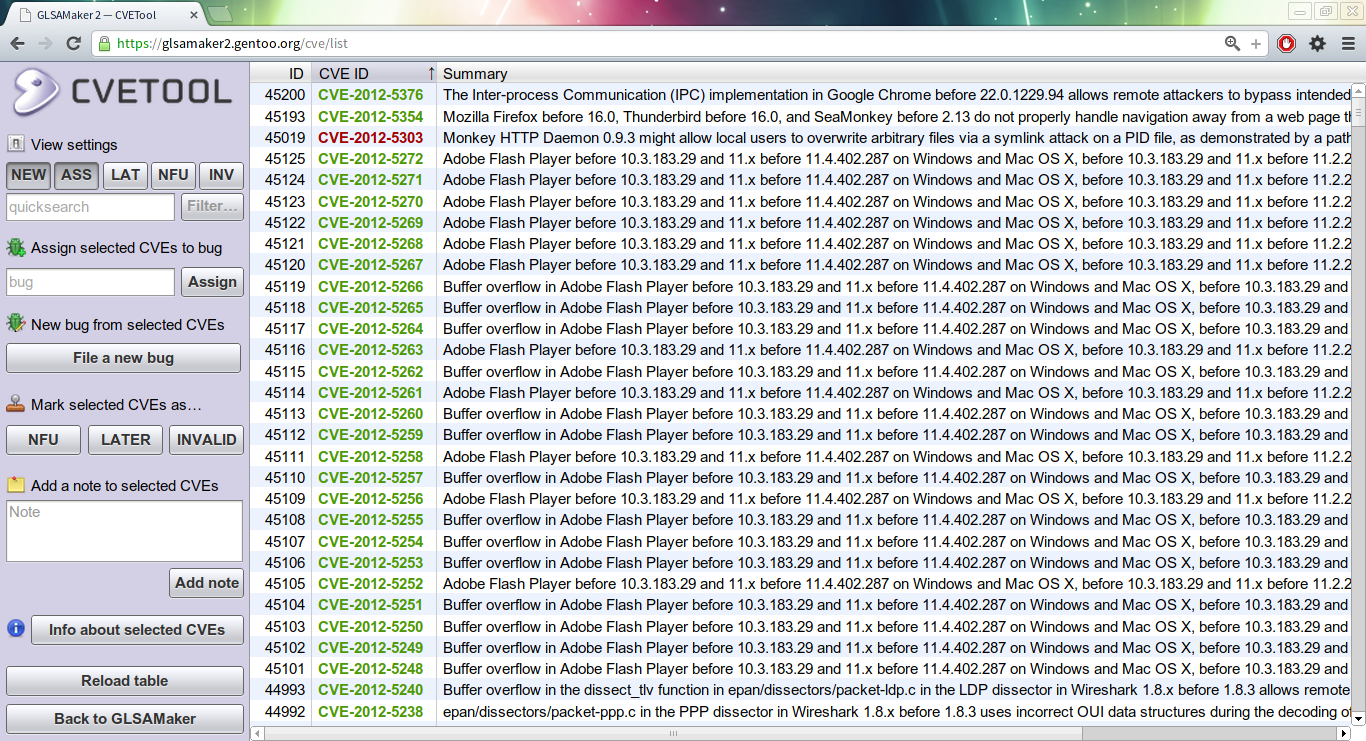
\includegraphics[width=0.9\paperwidth]{img/cvetool.png}   
    \end{figure}
  \end{changemargin}
\end{frame}

\begin{frame}
  \frametitle{Tools: GLSAMaker}
  \begin{changemargin}{-1cm}{-1cm}
    \begin{figure}
      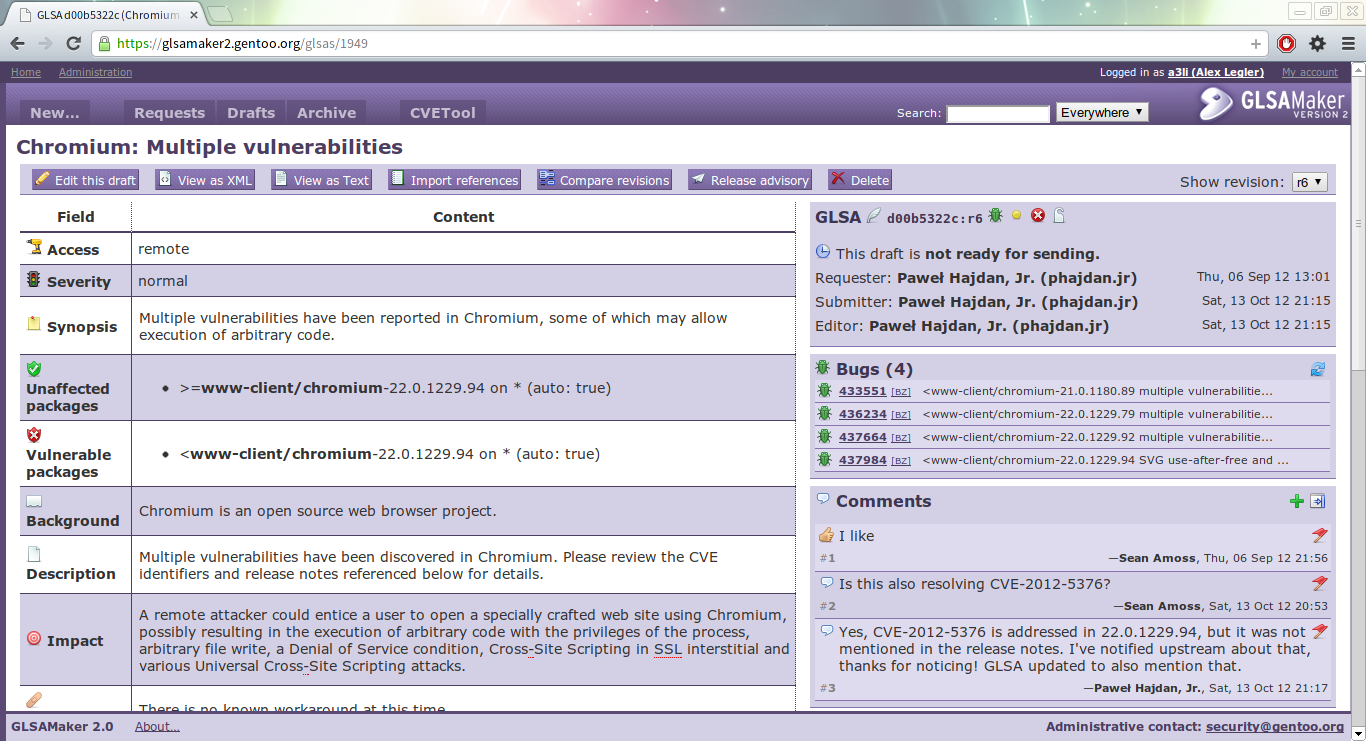
\includegraphics[width=0.9\paperwidth]{img/glsamaker.png}   
    \end{figure}
  \end{changemargin}
\end{frame}


\section{Keeping your system safe}
\subsection*{Keeping your system safe}

\begin{frame}[fragile]
  \frametitle{glsa-check}
  
  \begin{block}{Checking a system's overall GLSA status}
    \begin{Verbatim}[commandchars=\\\{\}]
\textcolor{gray}{$} \textbf{glsa-check -l affected}
[A] means this GLSA was marked as applied (injected),
\textcolor{gentoogreen}{[U]} means the system is not affected and
\textcolor{red}{[N]} indicates that the system might be affected.

\textcolor{red}{201209-03 [N]} PHP: Multiple vulnerabilities \(\hookleftarrow\)
 ( dev-lang/php )
\textcolor{red}{201209-13 [N]} libjpeg-turbo: Code execution \(\hookleftarrow\)
 ( media-libs/libjpeg-turbo )
\textcolor{red}{201209-14 [N]} file: Denial of Service \(\hookleftarrow\) 
 ( sys-apps/file )
    \end{Verbatim}
  \end{block}
\end{frame}

\begin{frame}[fragile]
  \frametitle{glsa-check (2)}
  
  \begin{block}{Finding an upgrade path}
    \begin{Verbatim}[commandchars=\\\{\}]
\textcolor{gray}{$} \textbf{glsa-check -p affected}
Checking GLSA 201209-13
>>> Updates that will be performed:
 \textcolor{gentoogreen}{media-libs/libjpeg-turbo-1.2.1} (vulnerable: \textcolor{red}{~-1.2.0})
Checking GLSA 201209-14
>>> Updates that will be performed:
 \textcolor{gentoogreen}{sys-apps/file-5.11} (vulnerable: \textcolor{red}{sys-apps/file-5.09})
Checking GLSA 201209-03
>>> No upgrade path exists for these packages:
 \textcolor{red}{dev-lang/php-5.3.15}
    \end{Verbatim}
  \end{block}
\end{frame}

\begin{frame}[fragile]
  \frametitle{glsa-check (3)}
  \begin{block}{Advisory details}
    \begin{Verbatim}[commandchars=\\\{\}]
\textcolor{gray}{$} \textbf{glsa-check -d 201206-27}
mini_httpd: Arbitrary code execution            
======================================================
Synopsis:  A vulnerability in mini_httpd could allow
           remote attackers to execute arbitrary code.
\dots
Resolution:Gentoo discontinued support for mini_httpd.
           We recommend that users unmerge mini_httpd:
           # emerge --unmerge "www-servers/mini_httpd"
    \end{Verbatim}
  \end{block}
\end{frame}

\begin{frame}
  \frametitle{Further efforts}
    \begin{itemize}\addtolength{\itemsep}{0.5\baselineskip}
     \item Gentoo Hardened
     \begin{itemize}
      \item Gentoo project offering various enhancements to the Kernel and Toolchain
      \item \url{http://hardened.gentoo.org/}
     \end{itemize}
     
     \item kernel-check
     \begin{itemize}
      \item Compares running kernel with a list of known issues
      \item Development stalled, volunteers wanted!
     \end{itemize}

     
     \item Security Auditing subproject
     \begin{itemize}
      \item Recent staff addition
      \item Gentoo will resume actively looking for issues
     \end{itemize}

    \end{itemize}
\end{frame}

\begin{frame}
  \frametitle{Future plans}
  
  \begin{itemize}\addtolength{\itemsep}{0.5\baselineskip}
    \item Getting Gentoo certified as \textit{CVE compatible}
    \item Updating GLSA format
      \begin{itemize}
        \item Less redundant information
        \item Slotting support
      \end{itemize}
    \item New \url{http://security.gentoo.org/}
    \begin{itemize}
      \item Searchable GLSA archive
      \item CVE–Package–GLSA mapping
      \item Notification service for medium/low severity issues without an advisory
    \end{itemize}
  \end{itemize}

\end{frame}


\section{Thanks}
\subsection*{Thanks}

\begin{frame}
  \frametitle{Thanks!}
  
  \begin{itemize}
    \item \textbf{Questions?}
  \end{itemize}

  \begin{itemize}
    \item Want to see the tools live? Ask me!
    \item The team can be reached via \href{mailto:security@gentoo.org}{\texttt{<security@gentoo.org>}}
  \end{itemize}

  %\hspace{.5em}
  \pause

  \begin{block}{Shameless plug: \alert{\textbf{We need your help!}}}
    \begin{itemize}
     \item File bugs you find or discover on \href{https://bugs.gentoo.org/}{\texttt{bugs.gentoo.org}}
     \item Help wrangle bugs
     \item Help draft, review and release advisories
     \item \textbf{Interested?} Contact us (now, not \textit{maybe later!})
    \end{itemize}

   
  \end{block}

\end{frame}

\begin{frame}
  \frametitle{Advertisement: Get Merchandise!}
  
  \begin{columns}[c]
    \column{.5\textwidth}
    
    \begin{figure}
      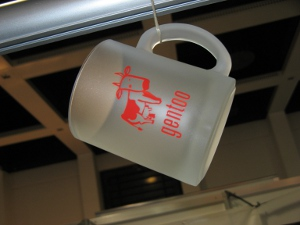
\includegraphics[width=0.9\textwidth]{img/gentoo_mug.jpg} 
    \end{figure}
    
    \column{.5\textwidth}
    
    \begin{itemize}
     \item Larry the cow mugs
     \item Available at the Gentoo booth
    \end{itemize}

  \end{columns}

\end{frame}

  
\end{document}
